\documentclass[a4paper, 12pt]{article}

\usepackage{cmap} % поиск в PDF
\usepackage[english, russian]{babel} % локализация и переносы
\parskip=3pt % дополнительное расстояние между абзацами
\usepackage{graphicx} % вставка рисунков
\usepackage{lastpage}
\usepackage{rotating}
%\usepackage{minted} % красивый код
%\usemintedstyle{friendly}

\usepackage{verbatim}
\usepackage{multirow} % Слияние строк в таблице
\usepackage{caption}
\usepackage{amsfonts, amssymb, amsthm, mathtools, amsmath} % AMS
\usepackage{array} % Дополнительная работа с таблицами
\usepackage{multicol}

%%% Цветной текст

\usepackage[usenames]{color}
\usepackage{colortbl}

%% Поля

\usepackage{geometry} 
\geometry{left=2cm}
\geometry{right=2cm}
\geometry{top=2cm}
\geometry{bottom=2cm}

%%% Гиперссылки

\usepackage[unicode]{hyperref}
\usepackage{xcolor}
\definecolor{urlcolor}{HTML}{4682B4} % цвет гиперссылок
\definecolor{linkcolor}{HTML}{4682B4} % цвет ссылок
\definecolor{citecolor}{HTML}{4682B4} % цвет библиоссылок
\hypersetup{pdfstartview=FitH,  linkcolor=linkcolor,urlcolor=urlcolor, citecolor=citecolor, colorlinks=true}

%% Немного дизайна

\definecolor{lb}{rgb}{0.8,0.85,1}
\renewcommand{\labelitemi}{$\diamond$}

\newcommand{\e}{\mathbb{E}}
\newcommand{\p}{\mathbb{P}}
\newcommand{\n}{\mathbb{N}}
\newcommand{\id}{\mathbb{I}}
\newcommand{\re}{\mathbb{R}}
\DeclareMathOperator{\plim}{plim}
\DeclareMathOperator{\var}{Var}
\DeclareMathOperator{\svar}{sVar}
\DeclareMathOperator{\argmin}{argmin}
\renewcommand{\epsilon}{\varepsilon}
\newcommand{\msum}{\sum\limits_1^n}
\newcommand{\isum}{\sum\limits_i^n}
\newcommand{\jsum}{\sum\limits_j^n}

\newcommand{\ds}{\displaystyle}

\begin{document}

\thispagestyle{empty}
\begin{center}
	\textbf{ПРАВИТЕЛЬСТВО РОССИЙСКОЙ ФЕДЕРАЦИИ}\\
	\vspace{3ex}
	\textbf{Федеральное государственное автономное\\ образовательное учреждение высшего образования}
	
	\vspace{3ex}
	
	\textbf{Национальный исследовательский университет \\ <<Высшая школа экономики>>}
	
	\vspace{10ex}
	\begin{flushright}
		Факультет экономических наук\\
		Образовательная программа <<Экономика>>
	\end{flushright}
\end{center}
\vspace{12ex}

\begin{center}
	{\textbf{КУРСОВАЯ РАБОТА
	}}
	\vspace{1ex}
	
	<<Методы интерпретации моделей машинного обучения>>
\end{center}
\vspace{4ex}
\begin{flushright}
	\noindent
	Студентка группы БЭК171\\Махнева Елизавета Александровна\\
	\vspace{13ex}
	Научный руководитель:\\
	Соколов Евгений Андреевич
	
\end{flushright}	

\vfill

\begin{center}
	Москва 2020
	
\end{center}
\newpage
	\tableofcontents
	\newpage
	
	\section{Введение}
	Во введении я хочу сказать про то что существует интерпретируемые и нет модели. Про то что нам хотелось бы интерпретировать и привести аргументы за (как минимум те 3 из презенташки). Наверное стоит объединить с блоком интерпретации, так как здесь особо больше нечего писать (если только много не получится), а воду лить не хочется

1. Интерпретируемые и нет модели. Желательно показать примеры, почему не интерпретируются.
2. Интерпретация нужна! Потому что...
3. Плюсы интерпретации и небольшие минусы
4. Что и как хотелось бы интерпретировать. Основы интерпретации -- какой она должна быть
5. Кратко перечислить методы, сказать какие они бывают
	\newpage
	
	\section{Методы интерпретации}
	\subsection{PDP}
	\textbf{PDP (Partial Dependence Plot, график частичной зависимости)} -- график, который показывает зависимость прогноза модели от значения отдельного признака. С его помощью мы можем понять, как некоторый признак влияет на предсказание. Данный график можно изобразить для двух либо трех признаков из имеющихся.

\subsubsection{Идея}
Визуализация -- это отличный способ интерпретации. Если мы хотим понять, как признаки влияют на результат, можно посмотреть, как меняется прогноз от изменения одного признака при прочих равных. В идеальной ситуации мы бы построили график зависимости результата от всех признаков и меняли бы только один. Однако мы сталкиваемся с проблемой: если признаков больше двух, построить график не получится. Поэтому чтобы сохранить возможность визуализации, можно анализировать зависимость результата от одного признака без учета влияния остальных, построив график зависимости от одного признака. Аналогично можно изучать влияние одновременно двух признаков, построив трехмерный график.

<Пример 2мерного и 3мерного графиков>
	\subsubsection{Принцип работы}
	Пусть $x = (x_1, \ldots, x_d)$ -- вектор признаков объекта. У нас есть модель $f(x): \re^d \rightarrow \re$. Мы хотим понять, как признаки $x_1$ и $x_2$ влияют на предсказание модели. Обозначим $x_r = (x_3, \ldots, x_d)$ за вектор остальных признаков.

Нам нужно получить функцию зависимости предсказания от одного-двух признаков при зафиксированных остальных: $g(x_1, x_2) = f(x_1, x_2 | \, x_r)$. % не знаю насколько корректно
Но если $x_1$ и/или $x_2$ зависимы с признаками из $x_r$, то возникает проблема. При изменении анализируемого признака меняется и зависимый с ним, который мы не рассматриваем -- мы не сможем рассмотреть чистый предельный эффект одного признака, на него всегда будет наложен эффект другого предиктора. Поэтому одной из предпосылок метода является независимость исследуемых признаков от остальных.

Но даже с предпосылкой о независимости признаков функция $g(x_1, x_2)$ не будет показывать точный результат, так как предельные эффекты предикторов разные для разных объектов выборки. Поэтому мы рассмотрим, как влияют анализируемые признаки на среднее предсказание. То есть найдем матожидание предсказания модели при фиксированных исследуемых признаках (как констант с точки зрения матожидания):

\[
\bar{g}(x_1, x_2) = \e(f(x_1, x_2, x_r) \, | x_r)
\]

Таким образом, мы получим функцию, которая показывает предельные эффекты признаков для среднего предсказания. Но чтобы найти матожидание, мы должны знать истинные распределения признаков. Поскольку нам недоступна данная информация, можно воспользоваться методом Монте-Карло, чтобы примерно оценить искомую функцию:

\[
\hat{g}(x_1, x_2) = \frac{1}{n} \isum f(x_1, x_2, X_r^{(i)}),
\]
где $X_r^{(i)}$ -- $i$ строка матрицы $X_r$, содержащей признаки $x_r$ для всех объектов выборки.
% не уверена что все красиво и понятно

Результат: функция показывает, как исследуемые признаки в среднем влияют на результат работы модели. Мы можем построить ее график, чтобы более наглядно посмотреть на влияние предикторов на предсказание.% не уверена что в среднем -- корректная формулировка

% добавить преимущества и недостатки


% почему бы просто эту функцию не находить
% способ дает меньшую точность там, где зависимость можно было достать из модели
% можно делать анимацию, если нельзя рассмотреть все сразу :)
% Должна быть предпосылка не о независимости случайных величин, а о том, что производная по исследуемому признаку не зависит от других величин -- возможно просто стоит написать, что обычно в моделях комбинации признаков не используются, а если и используются, то задаются извне пользователем. И если в этом способе используются какие-то комбинации даже этого признака с самим собой, и при этом они рассматриваются отдельно, то мне кажется этот метод будет бесполезен

% можно дополнить, что возможно стоит брать не матожидание, а предоставлять подставлять некоторые значения, потому что предельные эффекты все равно будут разные для всех -- например LIME так делает
	\subsubsection{Реализация}
	Реализации данных графиков есть в разных библиотеках: $\verb|pdpbox|$, $\verb|sklearn|$,\\ $\verb|(sklearn.inspection.plot_partial_dependence|$,\\ $\verb|sklearn.ensemble.partial_dependence.plot_partial_dependence)|$

Библиотека $\verb|pdpbox|$ предоставляет более аккуратное и более наглядное представление графиков. Инструкции по установке можно найти \href{https://github.com/SauceCat/PDPbox}{здесь}.

Попробуем самостоятельно построить несколько графиков. Для этого мы будем использовать \href{https://www.kaggle.com/ruchi798/movies-on-netflix-prime-video-hulu-and-disney}{датасет}, содержащий информацию о различных фильмах и сериалах, выходивших с 1900 года и по настоящее время на разных платформах. До построения графиков сделаем предобработку.

%\begin{minted}{Python}
%import pdpbox
%\end{minted}
	\subsection{LIME}
	LIME (Local Interpretable Model-Agnostic Explanations) -- метод, показывающий вклад признаков в отдельное предсказание, работающий с любой моделью.
% нужен ли перевод

\subsubsection{Идея}
Результаты некоторых моделей легко интерпретировать. Например, в линейной регрессии можно посмотреть на веса. Они показывают, насколько изменится предсказание при изменении признаков. Так для каждого конкретного предсказания можно понять, почему модель выдала именно такой результат -- виден непосредственный вклад каждого признака.

Но не все модели легко интерпретировать. Например, некоторые архитектуры нейронных сетей. Они зачастую значительно превосходят линейные модели, но при этом сама структура модели представляет собой <<черный ящик>> -- непонятно, как именно модель сформировала предсказание, какие признаки сильнее повлияли на решение нейронной сети.

Идея состоит в том, чтобы перенести свойство интерпретируемости простых моделей на более сложные. Мы можем обучить интерпретируемую модель по выборке, где ответами являются предсказания сложной модели. В процессе обучения модель анализирует зависимости непосредственно между признаками и предсказаниями сложной модели. Тогда мы сможем интерпретировать результаты простой модели, которые являются аппроксимацией предсказаний сложной.\\[2mm]
\begin{minipage}{0.57\linewidth}
\indent Возникает проблема: сложная модель выявляет зависимости, которые, например, линейная модель может не уловить. Идея данного метода заключается в том, чтобы обучать более простую модель в некоторой окрестности исследуемого объекта, предполагая что на очень локальном уровне нет сложных зависимостей. Например, дифференцируемые функции можно линеаризовать в окрестности заданной точки -- можно использовать линейную модель на локальном уровне.
\end{minipage}
\hspace{5mm}
\begin{minipage}{0.35\linewidth}
	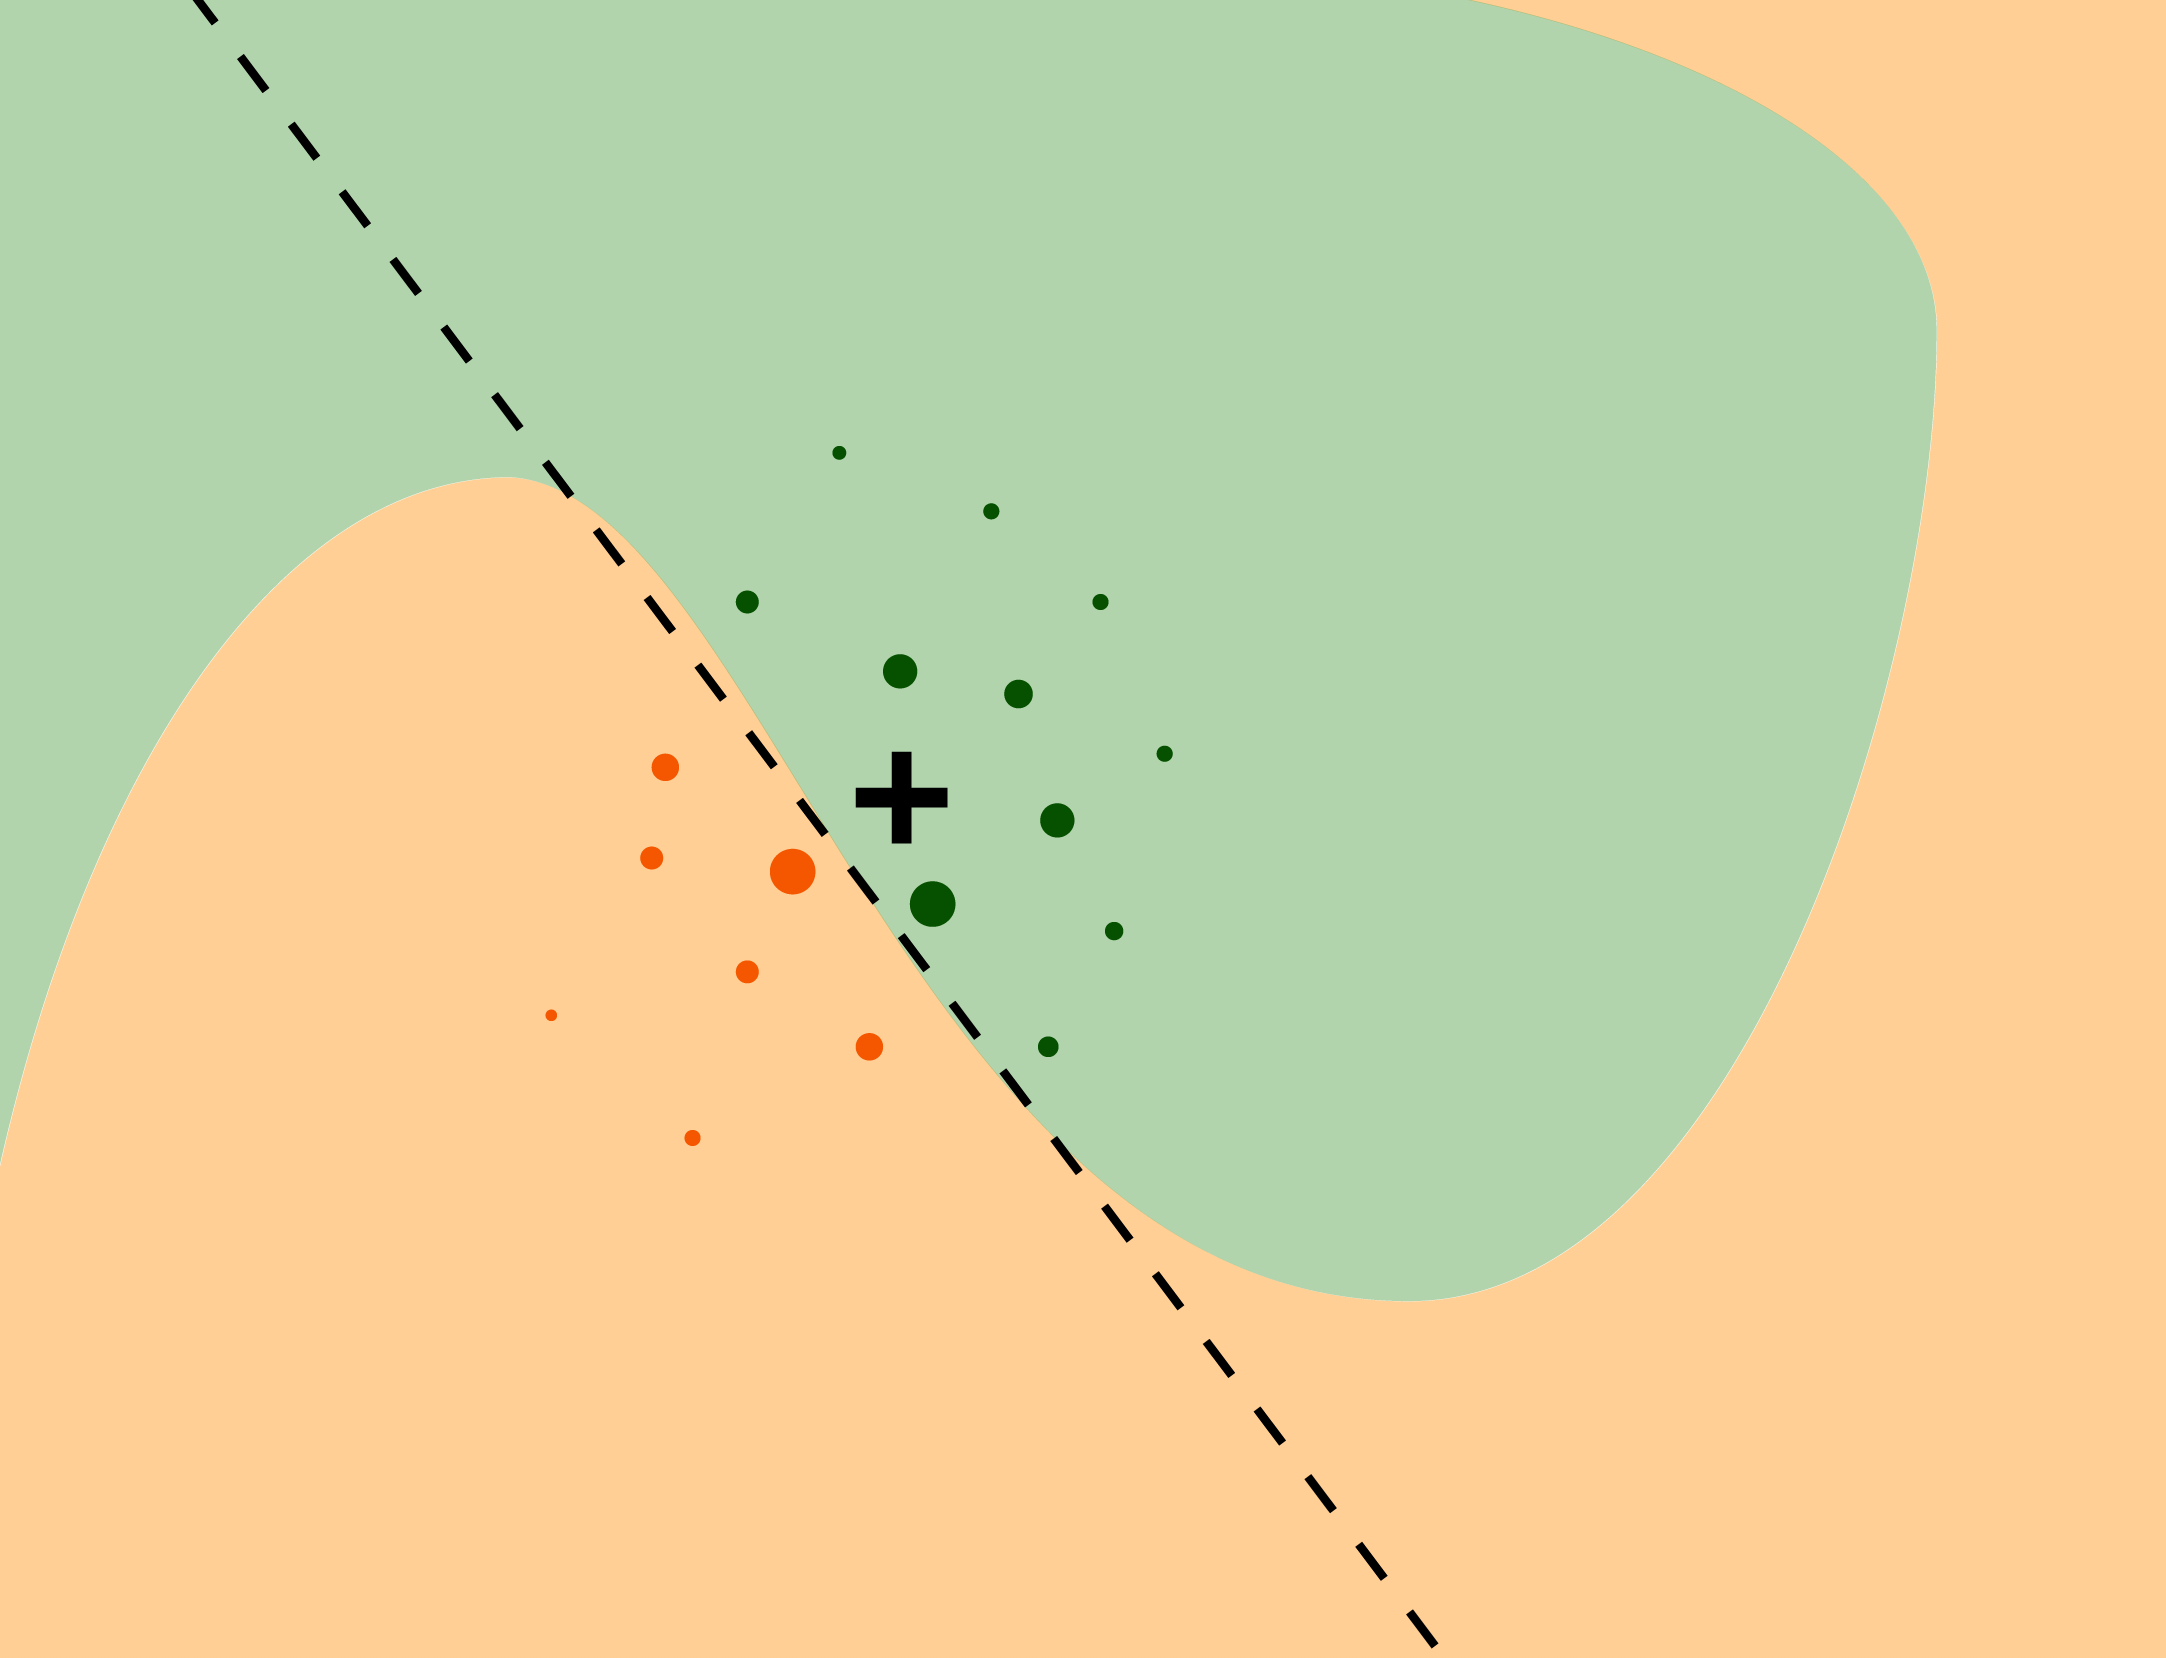
\includegraphics[width=6.5cm, height=5cm]{pics/lime4.png}
\end{minipage}

\underline{Пример LIME для табличных данных}
\vspace{-3mm}

\begin{figure}[h]
	\centering{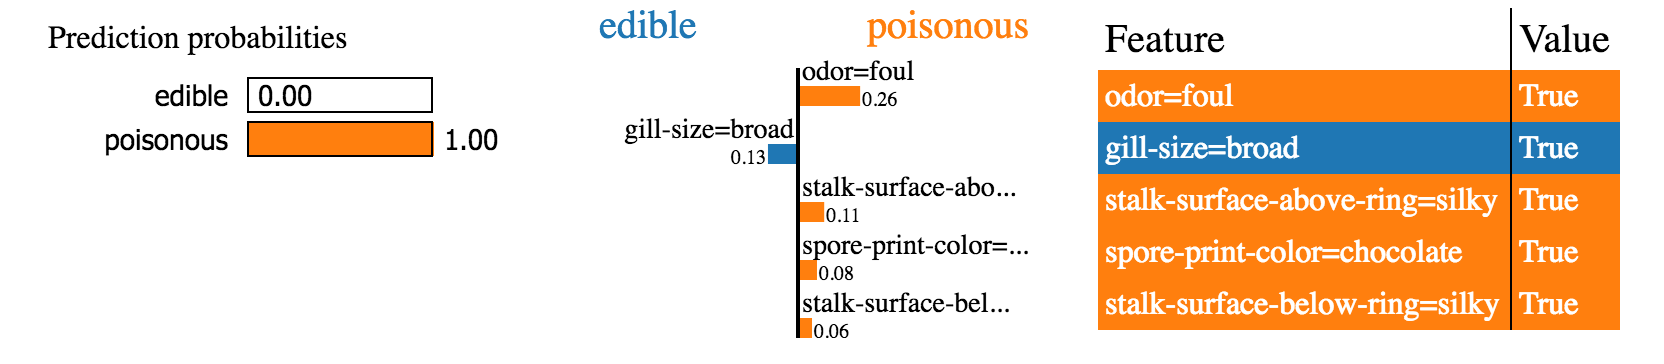
\includegraphics[width=\linewidth]{pics/lime1.png}}
\end{figure}

В данном случае решалась задача бинарной классификации. LIME вывел пять самых значимых признаков и показал, каким образом они повлияли на предсказание. Обученная модель показала, что исследуемый объект принадлежит к классу <<poisonous>>. И по анализу LIME понятно почему: только один признак из выведенных увеличил вероятность принадлежности объекта к классу <<edible>> и только на $0.13$. В то же время оставшиеся четыре признака повлияли на вероятность объекта быть <<poisonous>>, причем суммарно увеличив вероятность на $0.51$. Данная интерпретация позволяет понять, адекватна ли модель, которую мы получили, действительно ли релевантные признаки оказались значимыми.

\underline{Пример LIME для текстов}
\vspace{-3mm}

\begin{figure}[h]
	\centering{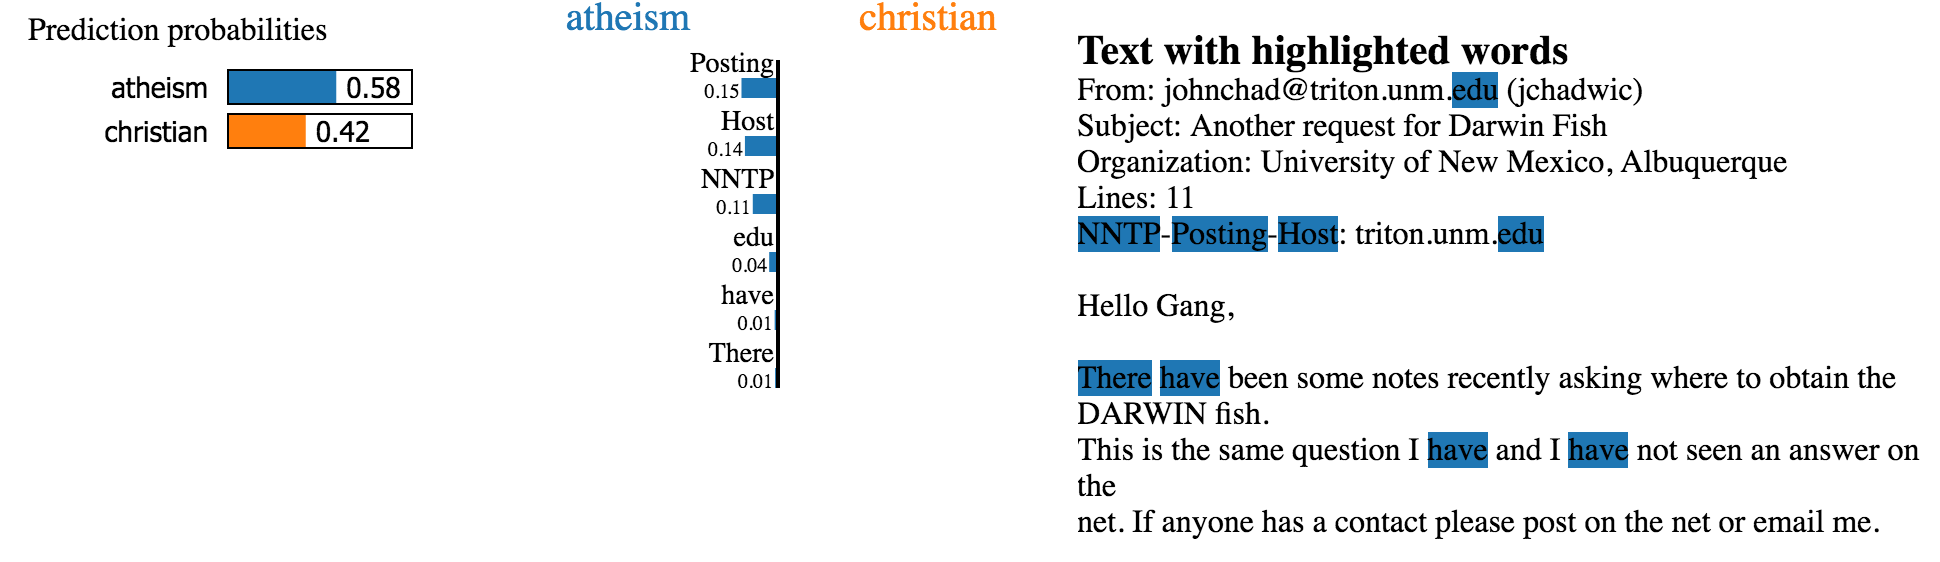
\includegraphics[width=\linewidth]{pics/lime2.png}}
\end{figure}

\underline{Пример LIME для картинок}
\vspace{-3mm}

\begin{figure}[h]
	\centering{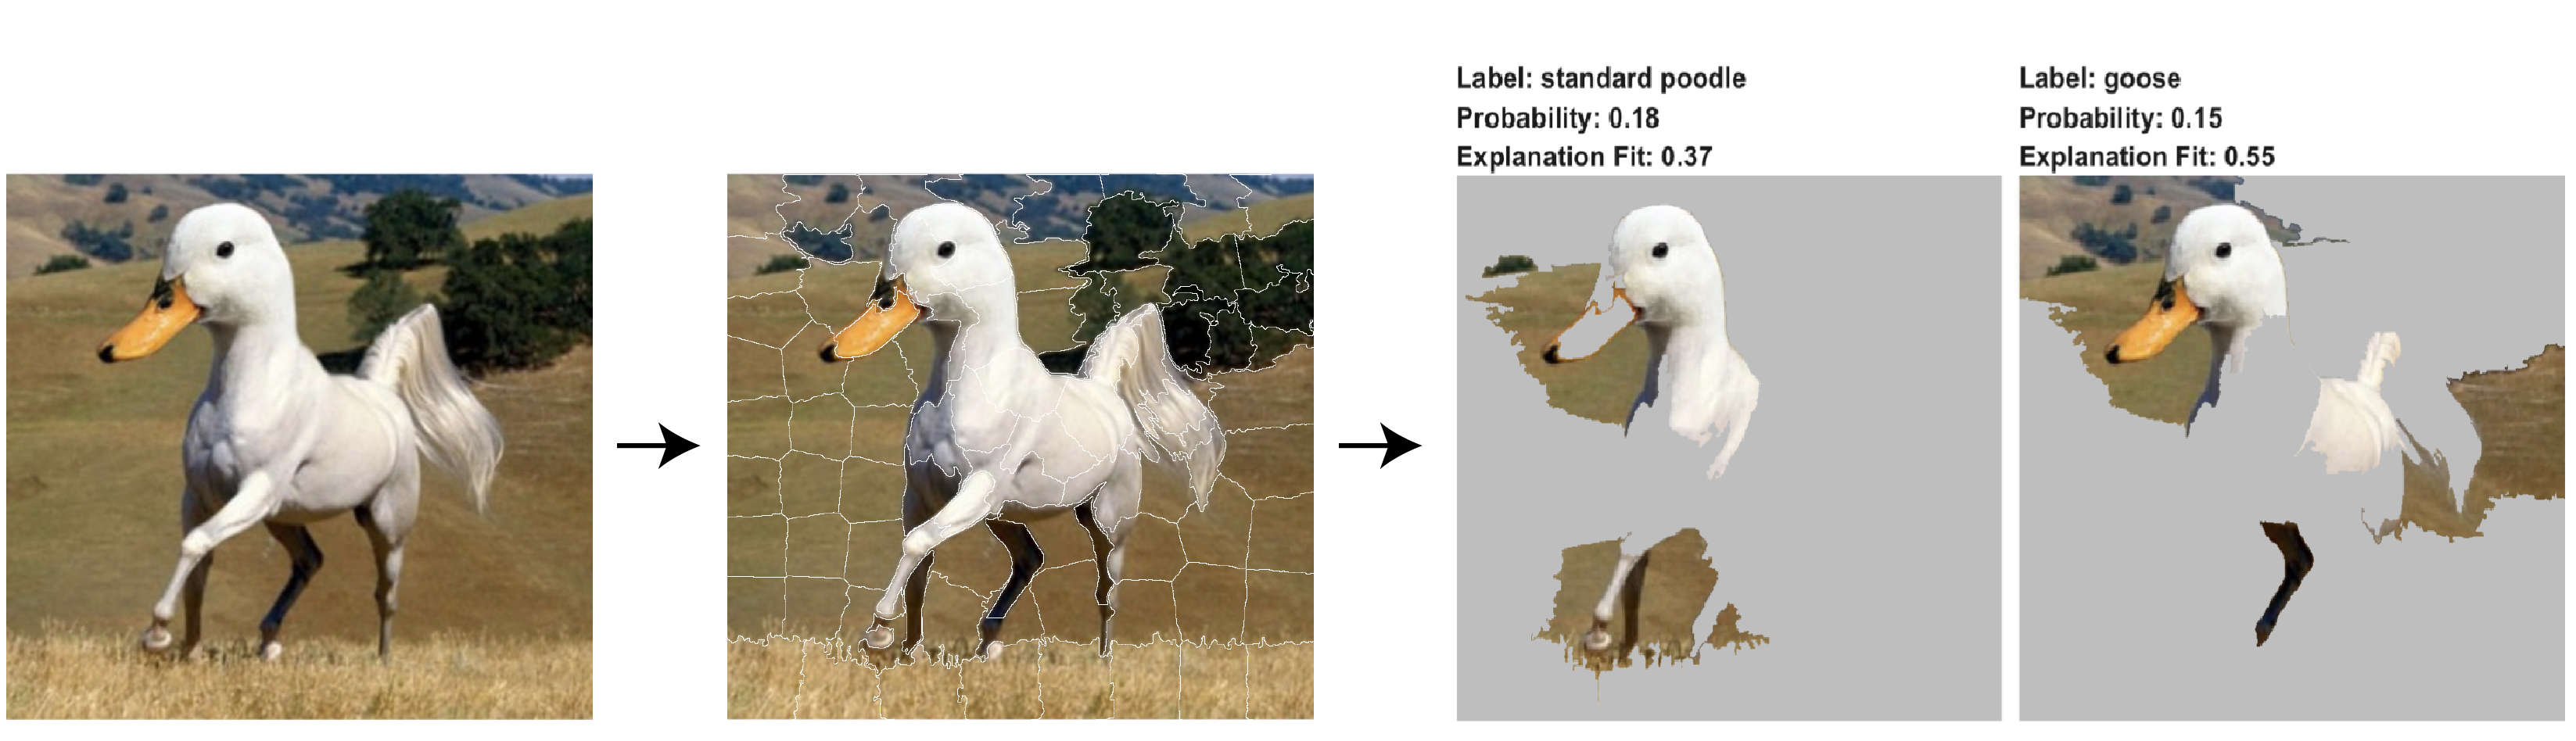
\includegraphics[width=\linewidth]{pics/lime3.png}}
\end{figure}

% почему не вытаскивать из самих моделей?
	\subsubsection{Принцип работы}
	У нас есть модель $f(x): \re^d \rightarrow \re$ и объект $x \in \re^d$, предсказание для которого нужно интерпретировать. Мы хотим найти модель $g$ из класса интерпретируемых моделей $G$, чтобы получить из нее объяснение результата более сложной модели (например, посмотреть на веса признаков).

Сложность моделей обычно обратно зависит от ее интерпретируемости. Например, линейную модель с 2-3 предикторами гораздо проще интерпретировать, чем модель с 10 и более предикторами. Поэтому нам нужно не просто использовать более простую модель, но и преобразовать исходное пространство признаков: $x \rightarrow x'$. Нам не подходят методы снижения размерности, которые представляют признаки в уже неинтерпретируемом виде (PCA, UMAP и пр.). В данной задаче можно уменьшить количество признаков и преобразовать их.

Чтобы уменьшить количество признаков, мы можем случайно выбирать некоторые из них. Либо комбинировать их между собой, при этом обращая внимание на интерпретируемость новых признаков. Для каждого типа данных подобное преобразование может проходить по-разному: для изображений -- несколько пикселей могут объединяться в один суперпиксель, для текстов -- символы объединяться в токены (например, слова -- они хорошо интерпретируются).

Для преобразования признаков существует большое количество методов. Например, приведение непрерывных переменных к дискретному виду. Основная цель подобных преобразований -- уменьшить множество значений признаков. Авторы алгоритма предлагают приводить предикторы к еще более упрощенному виду: использовать вместо признака дамми-переменную его наличия. Именно поэтому наша простая модель $g(x'):\{0,1\}^{d'} \rightarrow \re\,$ работает с интерпретируемым представлением предсказания $x' \in \{0,1\}^{d'}$, где обычно $d' << d$.
% что за бред, числовые переменные можно так и оставить, они же не мешают обучаться модели. или мешают
Дополнительно в задаче вводится мера сложности $\Omega(g)$ искомой модели как регуляризация. %Сложность модели может ограничиваться пользователем при регулировании гиперпараметров: глубина решающего дерева, количество моделей в ансамблях, количество слоев в нейронной сети и т.д.
% может быть здесь стоит писать все про интерпретируемые модели и не приводить такие примеры. Вообще не уверена что это нужна писать, здесь же мат часть

Чтобы определить окрестность рядом с $x$, внутри которой мы можем использовать простую модель, введем меру близости $\pi_x(z)$ между объектом $x$ и его соседом $z$. И наконец определим нашу функцию потерь, которую мы будем оптимизировать: $L(f, g, \pi_x)$ -- разница между моделями $f$ и $g$ в окрестности, заданной $\pi_x$. Тогда в целом задача алгоритма выглядит следующим образом:
\[
explanation(x) = \xi(x) = \underset{g \in G}{\argmin} (L(f, g, \pi_x) + \Omega(g))
\]

Одной из особенностей алгоритма является его независимость от модели, которую необходимо интерпретировать. Поэтому мы не можем приписывать модели $f$ никакие свойства. Вместо этого мы будем аппроксимировать ее, искусственно создавая объекты в окрестности $x'$, переводя их в исходное пространство признаков и получая для них предсказания из $f$.

Понятие окрестности носит абстрактный характер, поэтому чтобы учесть расстояние между объектами на практике, мы будем использовать меру близости $\pi_x(z)$ как веса: чем ближе объект к $x$, тем больший вклад он вносит в функцию потерь.

Гиперпараметры в задаче:\\[-8mm]
\begin{itemize}
	\item $G$ -- класс интерпретируемых моделей: линейные модели, решающие деревья и др.\\[-6mm]
	\item $d'$ -- количество признаков в новом пространстве
	\item $\pi_x(z)$ -- мера близости: например, ядра (гауссово, логистическое и др.)\\[-6mm]
	\item $D(x,z)$ -- расстояние между объектами, используемое при расчете меры близости: евклидова метрика, косинусное расстояние и др.\\[-6mm]
	\item $L$ -- функция потерь: $MSE$, $MAE$ и др.\\[-6mm]
\end{itemize}

% мне кажется процесс генерации новых объектов здесь не так важен
% у них еще есть тема с выбором примеров для объяснения модели -- пока что это не кажется важным
% непонятно что у них с простыми моделями -- они только линейные или нет
% есть гиперпараметр К

Результат: мы получаем алгоритм, который изучает работу более сложной модели и интерпретирует ее с некоторой погрешностью -- можно изучать влияние признаков на отдельные предсказания.

	\subsubsection{Реализация}
	Данный метод реализован в библиотеке $\verb|lime|$. Она содержит в себе методы для работы с разными типами данных: $\verb|lime.lime_tabular|$, $\verb|lime.lime_text|$, $\verb|lime.lime_image|$. Инструкцию по установке можно найти \href{https://github.com/marcotcr/lime}{здесь}.
	\subsection{SHAP}
	SHAP (SHapley Additive exPlanations) -- метод, оценивающий вклад признаков в предсказания модели на основе значений Шэпли.

\subsubsection{Идея}
Предсказание модели формируется на основе признаков. Если мы хотим узнать влияние отдельного признака, мы можем построить предсказание модели с ним и без него и затем посмотреть, как меняется результат. % почему реально не убирать насовсем?
Но модель может быть слишком сложной, чтобы мы могли оценить влияние предиктора по одному объекту, регулируя один признак при фиксированных остальных. % а корректно ли занулять его, это ведь тоже какое-то значение
% помнить про то, что у shapley values есть свой раздел
Правильнее рассмотреть все возможные комбинации признаков: их разные значения, наличие/отсутствие, чтобы понять, как в каждом из перечисленных случаев добавление и исключение признака влияет на предсказание.

Рассматривая влияние в каждом конкретном случае, мы получаем огромное количество предельных эффектов, что тяжело интерпретируется. Поэтому можно рассмотреть, какой в среднем эффект оказывает включение признака в модель. Тогда мы получим средневзвешенную оценку вклада отдельного признака в предсказание, что позволит проинтерпретировать результат работы модели.
% Подумать, почему они сравнивают результат со средним кроме как кроме того что нужна всего одна модель и теряется точность

Однако для такого способа нужно обучить количество моделей, равное количеству всех комбинаций признаков -- которое растет экспоненциально с увеличением количества признаков. Вместо этого мы можем аппроксимировать разницу между предсказаниями разных моделей разницей между предсказанием и ожидаемым предсказанием. % дописать идею

% мб метод SHAP вносит еще какие-то идеи, но пока что так

\subsubsection{Значения Шэпли (Shapley values)}
Для упрощения расчетов мы не будем рассматривать разные значения предикторов, а бинаризуем их представление, обозначив за <<1>> наличие предиктора и за <<0>> его отсутствие.
% наверняка можно как-то умнее упрощать признаки
% в чем отличие SHAP?
Тогда у нас есть некоторое ограниченное количество возможных комбинаций признаков. Пусть $S$ -- множество ненулевых признаков, в которое не входит исследуемый $i$-ый признак. Чтобы найти разницу предсказаний для признаков из $S$ и из $S \cup \{i\}$, куда входит $i$-ый признак, нам нужно обучить две модели, $f_S$ и $f_{S \cup \{i\}}$, соответственно. Тогда для объекта $x$ мы получим:
\[
f_{S \cup \{i\}}(x_{S \cup \{i\}}) - f_S(x_S),
\]

Как отмечалось ранее, значения данного выражения могут меняться при разных комбинациях признаков, поэтому мы усредним ее для всех возможных случаев. Считая, что $F$ -- множество всех признаков, получим итоговое выражение для $i$-го признака:
\[
\phi_i = \frac{1}{|F|} \sum\limits_{S \subseteq F \backslash \{i\}}
\begin{pmatrix}
|F| - 1 \\
|S|
\end{pmatrix}^{-1}
(f_{S \cup \{i\}}(x_{S \cup \{i\}}) - f_S(x_S)),
\]
где $|F|$ -- количество элементов в множестве $F$, $|S|$ -- в множестве $S$.

Коэффициент:
\[
\ds \begin{pmatrix}
|F| - 1 \\
|S|
\end{pmatrix} = \frac{(|F|-1)!}{|S|! \cdot (|F| - |S| - 1)!}
\]
равен количеству всех возможных комбинаций признаков без учета исследуемого. Поделив на него, а также на количество признаков получаем среднее значение вклада признака. % а зачем делить на колво признаков

Данный коэффициент также можно интерпретировать как вес комбинации при расчете среднего. Биномиальный коэффициент, равный количеству комбинаций, для одного или $|F|-1$ признаков меньше, чем для любого другого числа признаков. Соответственно, при делении на коэффициент мы получаем большее значение, который указывает на больший вес подобных комбинаций. Это имеет смысл, так как больше информации мы получаем, рассматривая влияние признаков по отдельности: либо оставляя только его, либо исключая все кроме него. С увеличением количества признаков в $S$ вес комбинации убывает.

Таким образом, мы получили величину, показывающую, какой в среднем вклад вносит конкретный признак в предсказание. Данное значение пришло из теории игр и носит название значение Шэпли (Shapley value). Они показывают, какой вклад внес в общий выигрыш отдельный игрок при кооперации. В нашей задаче мы рассматриваем предсказание модели как выигрыш, а признаки как игроков.
	\subsubsection{Принцип работы}
	Метод SHAP несколько отличается от использования значений Шэпли напрямую для интерпретации вклада признаков -- он модифицирует классический подход. Рассмотрим SHAP подробнее.

Вместо использования большого количества моделей мы обучим одну модель и далее будем пользоваться только ее предсказаниями. Тогда наша модель представима в виде $f: \re^d \rightarrow \re$. Вместо исключения из нее признаков (в таком случае нам пришлось бы переобучать модель) мы оставим данные признаки в виде случайных величин и посчитаем математическое ожидание предсказания при фиксированных включенных в модель признаках.

Для упрощения расчетов мы не будем рассматривать разные значения предикторов, а бинаризуем их представление, обозначив за <<1>> наличие предиктора и за <<0>> его отсутствие: $x \rightarrow x', \, x' = \{1\}^d$. % не знаю корректно ли
Обозначим за $z' \in \{0,1\}^d$ объект, у которого мы учитываем только признаки из $S$ при формировании предсказания:
$z_j =
\begin{cases}
1, \text{если $j \in S$}\\
0, \text{если $j \notin S$}\\
\end{cases}$.\\
То есть $z'$ -- одна из возможных комбинаций предикторов.

Обученная модель работает с исходным видом признаков, поэтому нам нужно также восстанавливать значения исходных признаков по бинарному вектору. Введем для этого функцию $h_x(z') = z$, где $x$ -- исходный вектор исследуемого объекта, $z'$ -- бинарный вектор, в котором некоторые признаки заменены нулями, $z$ -- представление вектора $z'$ в исходном пространстве признаков. Функция $h_x$ вместо единиц восстанавливает значения из вектора $x$, а вместо нулей оставляет признак как некоторую переменную (случайную величину).
% наверняка можно как-то умнее упрощать признаки
Тогда наше ожидаемое предсказание для $z$ представимо в виде математического ожидания:
\[
\bar{f}(z) = \e(f(z)|\,z_S)
\]

Мы знаем конкретные значения признаков $z_S$, так как функция $h_x$ перенесла их из объекта $x$. Найдя математическое ожидание мы можем подставить данные значения, чтобы получить условное математическое ожидание, которое и будет оценкой нашего предсказания. И уже данную формулу мы можем использовать при расчете необходимых значений.% здесь для его расчета мы почему-то переходили к безусловному матожиданию, это связано со свойствами значений Шэпли -- не уверена нужно ли это прописывать

Поскольку мы не знаем истинное распределение, чтобы иметь возможность посчитать матожидание, аппроксимируем его оценкой. Для этого немного изменим функцию $h_x$ -- теперь вместо нулей она будет проставлять случайные значения соответствующих признаков. Тогда для каждого множества $S$ мы сможем получить несколько предсказаний модели и усреднить их:
\[
\hat{f}(z) = \frac{1}{k} \sum\limits_{i=1}^k f(z_{F\backslash S}, z_S),
\]
где $z_{F\backslash S}$ -- исключенные из модели признаки, вместо которые подставлены случайные значения, $z_S$ -- включенные в модель признаки, значения которых известны из исследуемого объекта $x$.
\paragraph{Kernel SHAP.}% я очень хочу доказать то, что они доказали
Авторы алгоритма показали, что есть упрощенный способ найти значения Шэпли: % с оговоркой про то что это не значения Шэпли
с помощью взвешенного МНК. В нем аналогично перебираются разные комбинации $z'$ -- так формируется выборка $Z$ для регрессии. Зависимой переменной является предсказание модели для сгенерированной выборки (переведенной в исходное пространство признкаов): $y_i = f(h_x(z'_i)) = f(z_i)$, где $z'_i$ -- строка матрицы $Z$. Тогда решением нашей задачи является вектор: \[
\phi = (Z^T W Z)^{-1} Z^T W y
\] % нужно ли говорить про корреляцию признаков. они это указывают как раз при расчете условного матожидания, и здесь наверное аналогия в мультиколлинеарности, но это неточно

Чтобы коэффициенты в регрессии соответствовали искомым значения, веса должны быть заданы диагональной матрицей $W$: 
\[w_{ii}(z'_i) = \frac{|F|-1}{
	\begin{pmatrix}
	|F| \\
	|S_i|
	\end{pmatrix} \cdot |S_i| \cdot (|F| - |S_i|)} = \frac{|F|-1}{|F|} \cdot \frac{|S_i - 1|! \cdot (|F|-|S_i|-1)!}{(|F|-1)!},
\]
где $|S_i|$ -- количество элементов в множестве $S_i$, то есть количество ненулевых элементов в $z'_i$.

В данном случае коэффициент при константе будет показывать предсказание модели при отсутствии признаков. Коэффициенты при признаках являются соответствующими значениями Шэпли, % если так можно сказать. мб сноска
которые можно использовать для интерпретации их вклада в предсказание.

Ранее мы уже говорили о том, что комбинации, в которых либо почти все нули, либо почти все единицы имеют больший вес при расчете значений Шэпли. Данный факт сохраняется и в линейной регрессии, поэтому формируя выборку можно отдавать предпочтение именно данным примерам -- в случае, если мы ограничены в количестве наблюдений.

Интересно, что если записать задачу в более общем виде:
\[
\sum\limits_{z' \in Z} (f(h_x(z')) - g(z'))^2 \cdot \underbrace{\frac{|F|-1}{|F|} \cdot \frac{|S - 1|! \cdot (|F|-|S|-1)!}{(|F|-1)!}}_{w(z') = \pi_x(z')} = L(f, g, \pi_x) + \Omega(g) \rightarrow \min_g
\]

мы получим ровно ту же задачу, что решает LIME. То есть при определенных гиперпараметрах LIME и SHAP эквивалентны друг другу.
% регуляризация -- легально ли это, мы ведь хотим значения Шэпли хммм
% сказать что бесконечные веса -- я как-то устранила :О

Существуют и другие модификации SHAP: TreeSHAPLinear SHAP, Low-Order SHAP, Max SHAP, Deep SHAP. В отличие от классического подхода они специфицированы для отдельных классов моделей, что позволяет снизить время работы алгоритма.
% показать что графики похожи на PDP -- необязательно

% расписать разные виды SHAP, точно указать Tree

% нужно ли указывать свойства? я могу и без них доказать
% привести к тому, что они показывают отклонение от среднего -- объясняют его -- это осталось из основного источника -- не указала это -- это есть и в оригинальной статье -- добавлю, если смогу доказать
	\subsubsection{Реализация}
	Данный метод реализован в библиотеке $\verb|shap|$. Универсальный метод содержится в модуле: $\verb|shap.KernelExplainer|$. Модицикации перечисленные ранее являются более специлизированными:\\[-8mm]
\begin{itemize}
	\item $\verb|shap.TreeExplainer|$: XGBoost/LightGBM/CatBoost/scikit-learn/pyspark models\\[-7mm]
	\item $\verb|shap.DeepExplainer|$: TensorFlow/Keras models\\[-7mm]
	\item $\verb|shap.GradientExplainer|$: TensorFlow/Keras/PyTorch models\\[-7mm]
	\item и др.
\end{itemize}.

Инструкцию по установке можно найти \href{https://github.com/slundberg/shap}{здесь}.
	\newpage

	\section{Анализ данных и интерпретация}
	Рассмотрим описанные методы на конкретной задаче. Построим относительно сложную модель (градиентный бустинг) для бинарной классификации объектов. Помимо этого построим несколько интерпретируемых моделей (логистическая регрессия, решающее дерево), чтобы сравнить значимость, которую они придают предикторам, с анализом методов интерпретации.
	\subsection{Данные}
	Для анализа был выбран датасет, содержащий информацию о клиентах разных отелей за 2015-2017 года. Задача: предсказать, отменит ли клиент бронь. Датасет был предварительно обработан:
\begin{itemize}
	\item Удалены переменные company (много пропусков), reservation status, reservation status date (данная информация обычно бывает известна уже после отмены либо отъезда гостя)
	\item Приведены к числовому виду порядковые переменные meal, deposit type, arrival date month
	\item Удалены строки с пропущенными значениями -- таких строк было немного и в них была пропущена важная информация
\end{itemize}

Отдельн стоит отметить, что категориальные переменные reserved room type, assigned room type, hotel, country, market segment, distribution channel, customer type не были приведены к числовому виду, так как далее (спойлер) будет использоваться модель CatBoost, которая самостоятельно обрабатывает такие признаки.
	\subsection{Модели}
	Для анализа описанных методов я выбрала следующие модели: CatBoost (сложная модель), логистическая регрессия (простая интерпретируемая модель) и решающее дерево (простая интерпретируемая модель)

\paragraph{CatBoost.}
В первую очередь мне необходимо установить и импортировать данную библиотеку

$\verb|pip install catboost|$

$\verb|from catboost import CatBoostClassifier|$

\paragraph{LogisticRegression и DecisionTreeClassifier.}
Я буду использовать реализации данных моделей в $\verb|sklearn|$:

$\verb|from sklearn.linear_model import LogisticRegression|$

$\verb|from sklearn.tree import DecisionTreeClassifier|$

Обе модели имеют встроенные методы для извлечения важности признаков, поэтому будет легко интерпретировать их предсказания.
% здесь заметка про важность признаков у деревьев
	\subsection{Интерпретация результатов}
	Модель достигла неплохого качества в задаче классификации: ROC-AUC=0.9, accuracy=0.82. Попробуем интерпретировать ее результаты.

Нулевой способ это встроенный метод XGBoost, показывающий важность признаков при предсказании. Посмотрим на первые 5 самых важных признаков. Данная величина может быть расчитана тремя способами: <<weight>>, <<gain>>, <<cover>>. Первый показывает, сколько раз признак появляется в дереве:

\begin{figure}[h]
	\centering{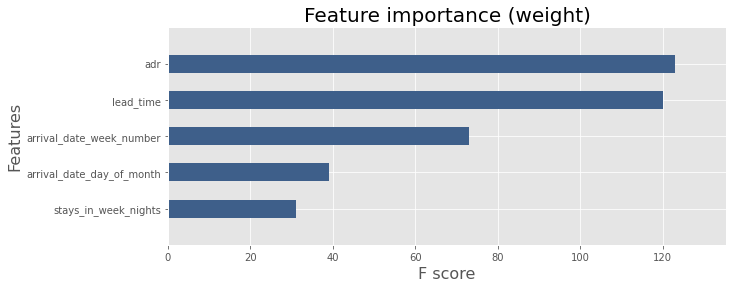
\includegraphics[width=0.85\linewidth]{pics/imp1.png}}
\end{figure}

Второй -- на сколько в среднем уменьшалась ошибка при использовании данного признака:

\begin{figure}[h]
	\centering{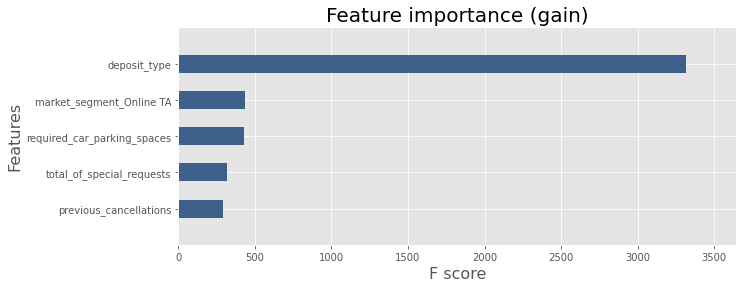
\includegraphics[width=0.85\linewidth]{pics/imp2.png}}
\end{figure}

И последний -- какое количество объектов выборки задействовало узлы с заданным признаком:

\begin{figure}[h]
	\centering{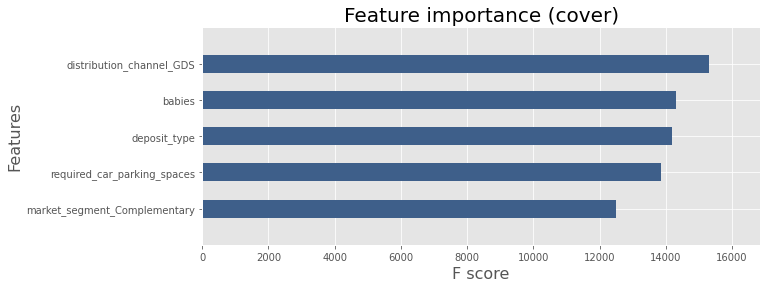
\includegraphics[width=0.85\linewidth]{pics/imp3.png}}
\end{figure}

Теперь перейдем к описанным ранее методам. Первый -- PDP. Возьмем признаки, которые сам XGBoost посчитал наиболее важными: первые два из weight (adr, lead\_time), первый из gain (deposit\_type) и первый из cover (distribution\_channel\_GDS) -- они с отрывом вырываются в лидеры.

И также возьмем признаки, которые XGBoost счел самыми незначительными: последний из weight (distribution\_channel\_GDS, забавно -- в тренировочной выборке всего 145 объектов, которым соответствует GDS. Судя по всему данный признак встречается 1-2 раза в узлах деревьев, но при этом он отсекает очень много объектов, из-за чего cover считает его важным), последние два из gain (customer\_type\_group, market\_segment\_Direct) и последний из cover (market\_segment\_Offline TA/TO).

Построим для них PDP. % на непрерывные как-то поадекватнее смотреть

\begin{tabular}{c|c}
	\arrayrulecolor[rgb]{0.8,0.85,1}
	\includegraphics*[width = 0.47\textwidth]{pics/mypdp1.png} & \includegraphics*[width = 0.47\textwidth]{pics/mypdp2.png}\\
	\hline
%	\includegraphics*[width = 0.5\textwidth]{mypdp3.png} & \includegraphics*[width = 0.5\textwidth]{mypdp4.png}}\\
%	\hline
%	\includegraphics*[width = 0.5\textwidth]{mypdp5.png} & \includegraphics*[width = 0.5\textwidth]{mypdp6.png}\\
%	\hline
%	\includegraphics*[width = 0.5\textwidth]{mypdp7.png} & \includegraphics*[width = 0.5\textwidth]{mypdp8.png}\\
\end{tabular}\\[2mm]
	\newpage
	
	\section{Заключение}
	Таким образом, существующие методы интерпретации моделей машинного обучения показывают неплохие результаты. Безусловно, они имеют свои недостатки, но несмотря на это они справляются со своей задачей и с некоторой погрешностью объясняют работу сложных моделей.
	\newpage
	
	\begin{thebibliography}{99}
		\bibitem{basis}
		\href{https://christophm.github.io/interpretable-ml-book/}{Interpretable Machine Learning | Christoph Molnar | Christoph Molnar | 2020 | all pages}
		\bibitem{LIME}
		\href{https://arxiv.org/pdf/1602.04938.pdf}{“Why Should I Trust You?” Explaining the Predictions of Any Classifier
| ...}
	\end{thebibliography}
	\newpage
	
	\section{Приложения}
	\paragraph{Приложение 1.}\label{sec:app1} Описание данных:

\end{document}